% ==============================================================================
% =================================== Aufgabe 1 ================================
% ==============================================================================

\chapter{Aufgabe (1)}
\label{chap:Aufgabe1}
\thispagestyle{fancy}

Die folgende Aufgabe basiert auf dem Datensatz \texttt{movies2019.csv}, der die im Jahr 2019 erschienenen Filme mit ihren Distributoren, Genres und Umsätzen enthält.

% ======================================= a =====================================

\section{Daten einlesen und erste fünf Zeilen anzeigen (a)}
\label{sec:1a}

\subsection{Aufgabenstellung}

Der Datensatz \texttt{movies2019.csv} wird in einen \texttt{Pandas DataFrame} eingelesen und die ersten fünf Zeilen werden angezeigt.

\subsection{Lösung}

Der Datensatz wird mit der Pandas-Funktion \texttt{read\_csv()} eingelesen. Die Methode \texttt{head()} gibt die ersten fünf Zeilen zurück, um einen ersten Eindruck von der Struktur der Daten zu gewinnen.

\lstinputlisting[
    language=Python, 
    caption={Daten einlesen und erste fünf Zeilen anzeigen}, 
    label={lst:aufgabe1a}
]{asset/code/Aufgabe1a.tex}

\subsection{Ausgabe}

Die Ausgabe zeigt die ersten fünf Zeilen des Datensatzes mit den Spalten \texttt{Rank}, \texttt{Movie}, \texttt{Release Date}, \texttt{Distributor}, \texttt{Genre}, \texttt{2019 Gross} und \texttt{Tickets Sold}:

\begin{verbatim}
   Rank                      Movie  Release Date    Distributor      Genre  \
0     1          Avengers: Endgame  Apr 26, 2019    Walt Disney     Action   
1     2             Captain Marvel   Mar 8, 2019    Walt Disney     Action   
2     3                Toy Story 4  Jun 21, 2019    Walt Disney  Adventure   
3     4              The Lion King  Jul 19, 2019    Walt Disney  Adventure   
4     5  Spider-Man: Far From Home   Jul 2, 2019  Sony Pictures     Action   

     2019 Gross Tickets Sold  
0  $857,190,335   94,093,340  
1  $426,829,839   46,852,891  
2  $404,979,743   44,454,417  
3  $403,748,078   44,319,218  
4  $354,788,925   38,944,997
\end{verbatim}

\subsection{Interpretation}

Der Datensatz wird mit \texttt{pd.read\_csv()} eingelesen und in der Variablen \texttt{df} gespeichert. Die Methode \texttt{df.head()} gibt die ersten fünf Zeilen als DataFrame zurück und ermöglicht eine erste strukturelle Inspektion der Daten. Die Ausgabe zeigt sieben Spalten, darunter \texttt{Rank}, \texttt{Movie}, \texttt{Distributor}, \texttt{Genre}, \texttt{2019 Gross} und \texttt{Tickets Sold}. Bereits in den ersten fünf Zeilen ist erkennbar, dass die Top-Filme des Jahres 2019 aus den Genres \texttt{Action} und \texttt{Adventure} stammen.

\cleardoublepage

% ======================================= b =====================================

\section{Count Plot der Spalte ``Genre'' (b)}
\label{sec:1b}

\subsection{Aufgabenstellung}

Für die Spalte \texttt{Genre} wird ein Count Plot erstellt, der die Häufigkeitsverteilung der verschiedenen Genres visualisiert.

\subsection{Lösung}

Zur Visualisierung wird die Bibliothek \texttt{seaborn} verwendet. Der Count Plot wird mit der Funktion \texttt{sns.countplot()} erstellt. Die Plot-Größe wird mit \texttt{plt.figure(\textit{figsize=(12,6)})} angepasst, um eine gute Lesbarkeit der Genre-Bezeichnungen zu gewährleisten. Die X-Achsen-Beschriftungen werden zur besseren Übersicht um 45 Grad gedreht.

\lstinputlisting[
    language=Python, 
    caption={Count Plot der Spalte ``Genre''}, 
    label={lst:aufgabe1b}
]{asset/code/Aufgabe1b.tex}

\subsection{Ausgabe}

Die Ausgabe zeigt die Häufigkeitsverteilung der Genres im Datensatz:

\begin{figure}[h]
    \centering
    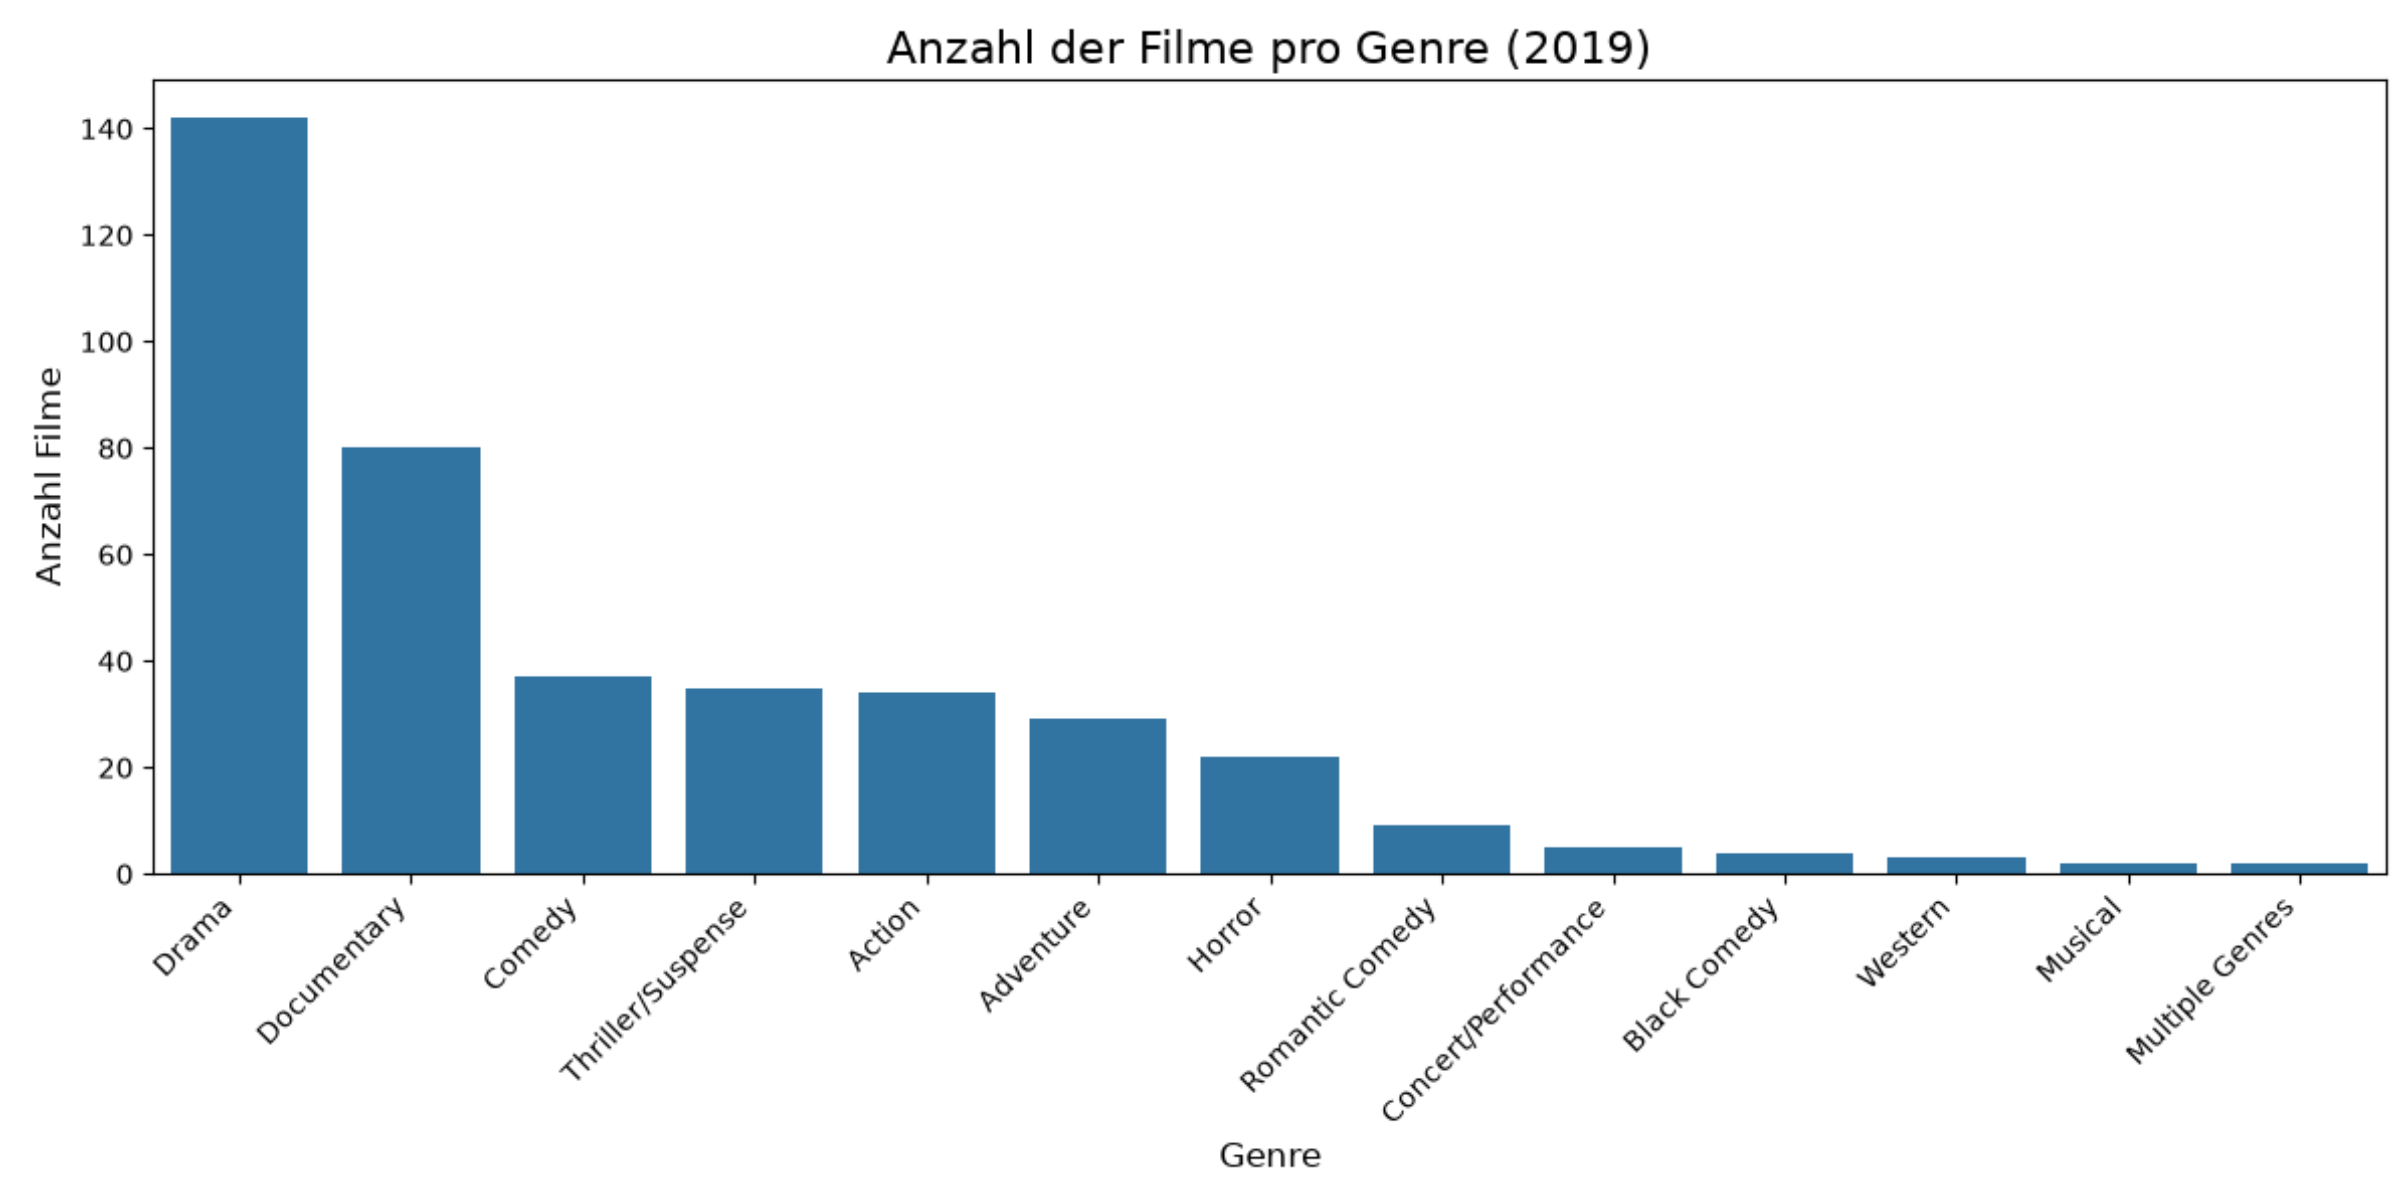
\includegraphics[width=0.9\textwidth]{./asset/image/Aufgabe1b.png}
    \caption{Count Plot der Spalte ``Genre'' (\textit{Quelle: Eigene Darstellung})}
    \label{fig:aufgabe1b}
\end{figure}

\subsection{Interpretation}

Der Count Plot visualisiert die Anzahl der Filme pro Genre. Dazu wird \texttt{sns.countplot()} mit der Spalte \texttt{Genre} als X-Achse verwendet. Die Sortierung der Balken erfolgt absteigend nach Häufigkeit mittels \verb|order=df['Genre'].value_counts().index|, wodurch das Genre mit den meisten Filmen zuerst dargestellt wird.

\cleardoublepage

% ======================================= c =====================================

\section{Konvertierung der Spalte ``2019 Gross'' und Berechnung des Gesamtumsatzes (c)}
\label{sec:1c}

\subsection{Aufgabenstellung}

Die Spalte \texttt{2019 Gross} liegt als String vor (\textit{\acs{z. B.} \texttt{\$857,190,335}}). Sie wird in numerische Werte konvertiert, um weitere Berechnungen zu ermöglichen. Anschließend wird der Gesamtumsatz aller Filme des Jahres 2019 ermittelt.

\subsection{Lösung}

Zur Konvertierung wird eine eigene Funktion \texttt{convert\_gross()} definiert, die mit \texttt{apply()} auf die Spalte \texttt{2019 Gross} angewendet wird. Die Funktion entfernt die Zeichen \texttt{\$} und \texttt{M} sowie Kommas und konvertiert den verbleibenden String in einen Float-Wert. Der Gesamtumsatz wird durch Summation der konvertierten Spalte mit \texttt{sum()} berechnet.

\lstinputlisting[
    language=Python, 
    caption={Konvertierung der Spalte ``2019 Gross'' und Berechnung des Gesamtumsatzes}, 
    label={lst:aufgabe1c}
]{asset/code/Aufgabe1c.tex}

\subsection{Ausgabe}

Die Ausgabe zeigt den Gesamtumsatz aller Filme des Jahres 2019:

\begin{verbatim}
Gesamtumsatz 2019: $6,786,167,073.00 Millionen
\end{verbatim}

\subsection{Interpretation}

Die Spalte \texttt{2019 Gross} wird mit \texttt{apply()} und einer benutzerdefinierten Funktion \texttt{convert\_gross()} von einem String in einen numerischen Wert konvertiert. Die Funktion entfernt zunächst alle nicht-numerischen Zeichen (\textit{\texttt{\$}, \texttt{M}, Kommas}) und wandelt den bereinigten String in einen Float um. Diese Vorgehensweise ermöglicht die weitere numerische Verarbeitung der Umsatzdaten. Der Gesamtumsatz wird durch Anwendung von \texttt{sum()} auf die konvertierte Spalte berechnet.

\cleardoublepage

% ======================================= d =====================================

\section{Summenstatistik nach Genre (d)}
\label{sec:1d}

\subsection{Aufgabenstellung}

Für die Spalte \texttt{2019 Gross} wird eine Summenstatistik nach Genre erstellt. Die Statistik umfasst die Anzahl der Filme pro Genre sowie den Gesamtumsatz pro Genre. Außerdem werden die Genres mit den meisten und den wenigsten Filmen ermittelt.

\subsection{Lösung}

Die Gruppierung erfolgt mit der Methode \texttt{groupby()} auf der Spalte \texttt{Genre}. Die Aggregation wird mit \texttt{agg(\textit{['count', 'sum']})} durchgeführt, um sowohl die Anzahl der Filme als auch den Gesamtumsatz pro Genre zu berechnen. Die Sortierung erfolgt absteigend nach der Anzahl der Filme mit \texttt{sort\_values()}. Die Genres mit den meisten und den wenigsten Filmen werden durch Zugriff auf den ersten und letzten Index der sortierten Tabelle ermittelt.

\lstinputlisting[
    language=Python, 
    caption={Summenstatistik nach Genre}, 
    label={lst:aufgabe1d}
]{asset/code/Aufgabe1d.tex}

\subsection{Ausgabe}

Die Ausgabe zeigt die Summenstatistik nach Genre sowie die Genres mit den meisten und den wenigsten Filmen:

\begin{verbatim}
Summenstatistik nach Genre:
                     Anzahl Filme  Gesamtumsatz (Mio)
Genre                                                
Drama                         142    $541,483,413.00M
Documentary                    80     $60,283,496.00M
Comedy                         37    $518,142,283.00M
Thriller/Suspense              35    $542,834,290.00M
Action                         34  $2,436,683,565.00M
Adventure                      29  $2,151,730,471.00M
Horror                         22    $375,969,919.00M
Romantic Comedy                 9     $81,761,874.00M
Concert/Performance             5      $1,758,562.00M
Black Comedy                    4     $36,609,765.00M
Western                         3      $1,707,418.00M
Multiple Genres                 2      $3,545,060.00M
Musical                         2     $33,582,542.00M

Die meisten Filme: Drama (142 Filme)
Die wenigsten Filme: Musical (2 Filme)
\end{verbatim}

\subsection{Interpretation}

Die Gruppierung erfolgt mit \texttt{groupby()} auf der Spalte \texttt{Genre}. Die Methode \texttt{agg(\textit{['count', 'sum']})} berechnet gleichzeitig die Anzahl der Filme pro Genre (\textit{\texttt{count}}) und den Gesamtumsatz pro Genre (\textit{\texttt{sum}}). Die Sortierung mit \texttt{sort\_values(\textit{ascending=False})} ordnet die Genres absteigend nach der Anzahl der Filme. Durch Zugriff auf den ersten (\textit{\texttt{index[0]}}) und letzten (\textit{\texttt{index[-1]}}) Eintrag der sortierten Tabelle werden die Genres mit den meisten und den wenigsten Filmen ermittelt.

\cleardoublepage

% ======================================= e =====================================

\section{Barplot: Gesamtumsatz pro Genre (e)}
\label{sec:1e}

\subsection{Aufgabenstellung}

Es wird ein Barplot erstellt, der den Gesamtumsatz pro Genre visualisiert. Auf der x-Achse werden die Genres, auf der y-Achse der Gesamtumsatz dargestellt. Die Plot-Größe wird an die Anzahl der Genres angepasst.

\subsection{Lösung}

Zur Visualisierung wird die Bibliothek \texttt{seaborn} verwendet. Zunächst werden die Daten mit \texttt{groupby()} nach Genre gruppiert und die Summe des Umsatzes pro Genre berechnet. Der Barplot wird mit \texttt{sns.barplot()} erstellt, wobei die Genres auf der x-Achse und die Umsätze auf der y-Achse abgetragen werden. Die Sortierung erfolgt absteigend nach Umsatz mit \texttt{sort\_values(\textit{ascending=False})}. Die Plot-Größe wird mit \texttt{figsize=(\textit{14,7})} angepasst. Zusätzlich werden die Umsatzwerte über den Balken mit \texttt{plt.text()} eingeblendet, um die Lesbarkeit zu verbessern.

\lstinputlisting[
    language=Python, 
    caption={Barplot: Gesamtumsatz pro Genre}, 
    label={lst:aufgabe1e}
]{asset/code/Aufgabe1e.tex}

\subsection{Ausgabe}

Die Ausgabe zeigt den Gesamtumsatz pro Genre als Balkendiagramm:

\begin{figure}[h]
    \centering
    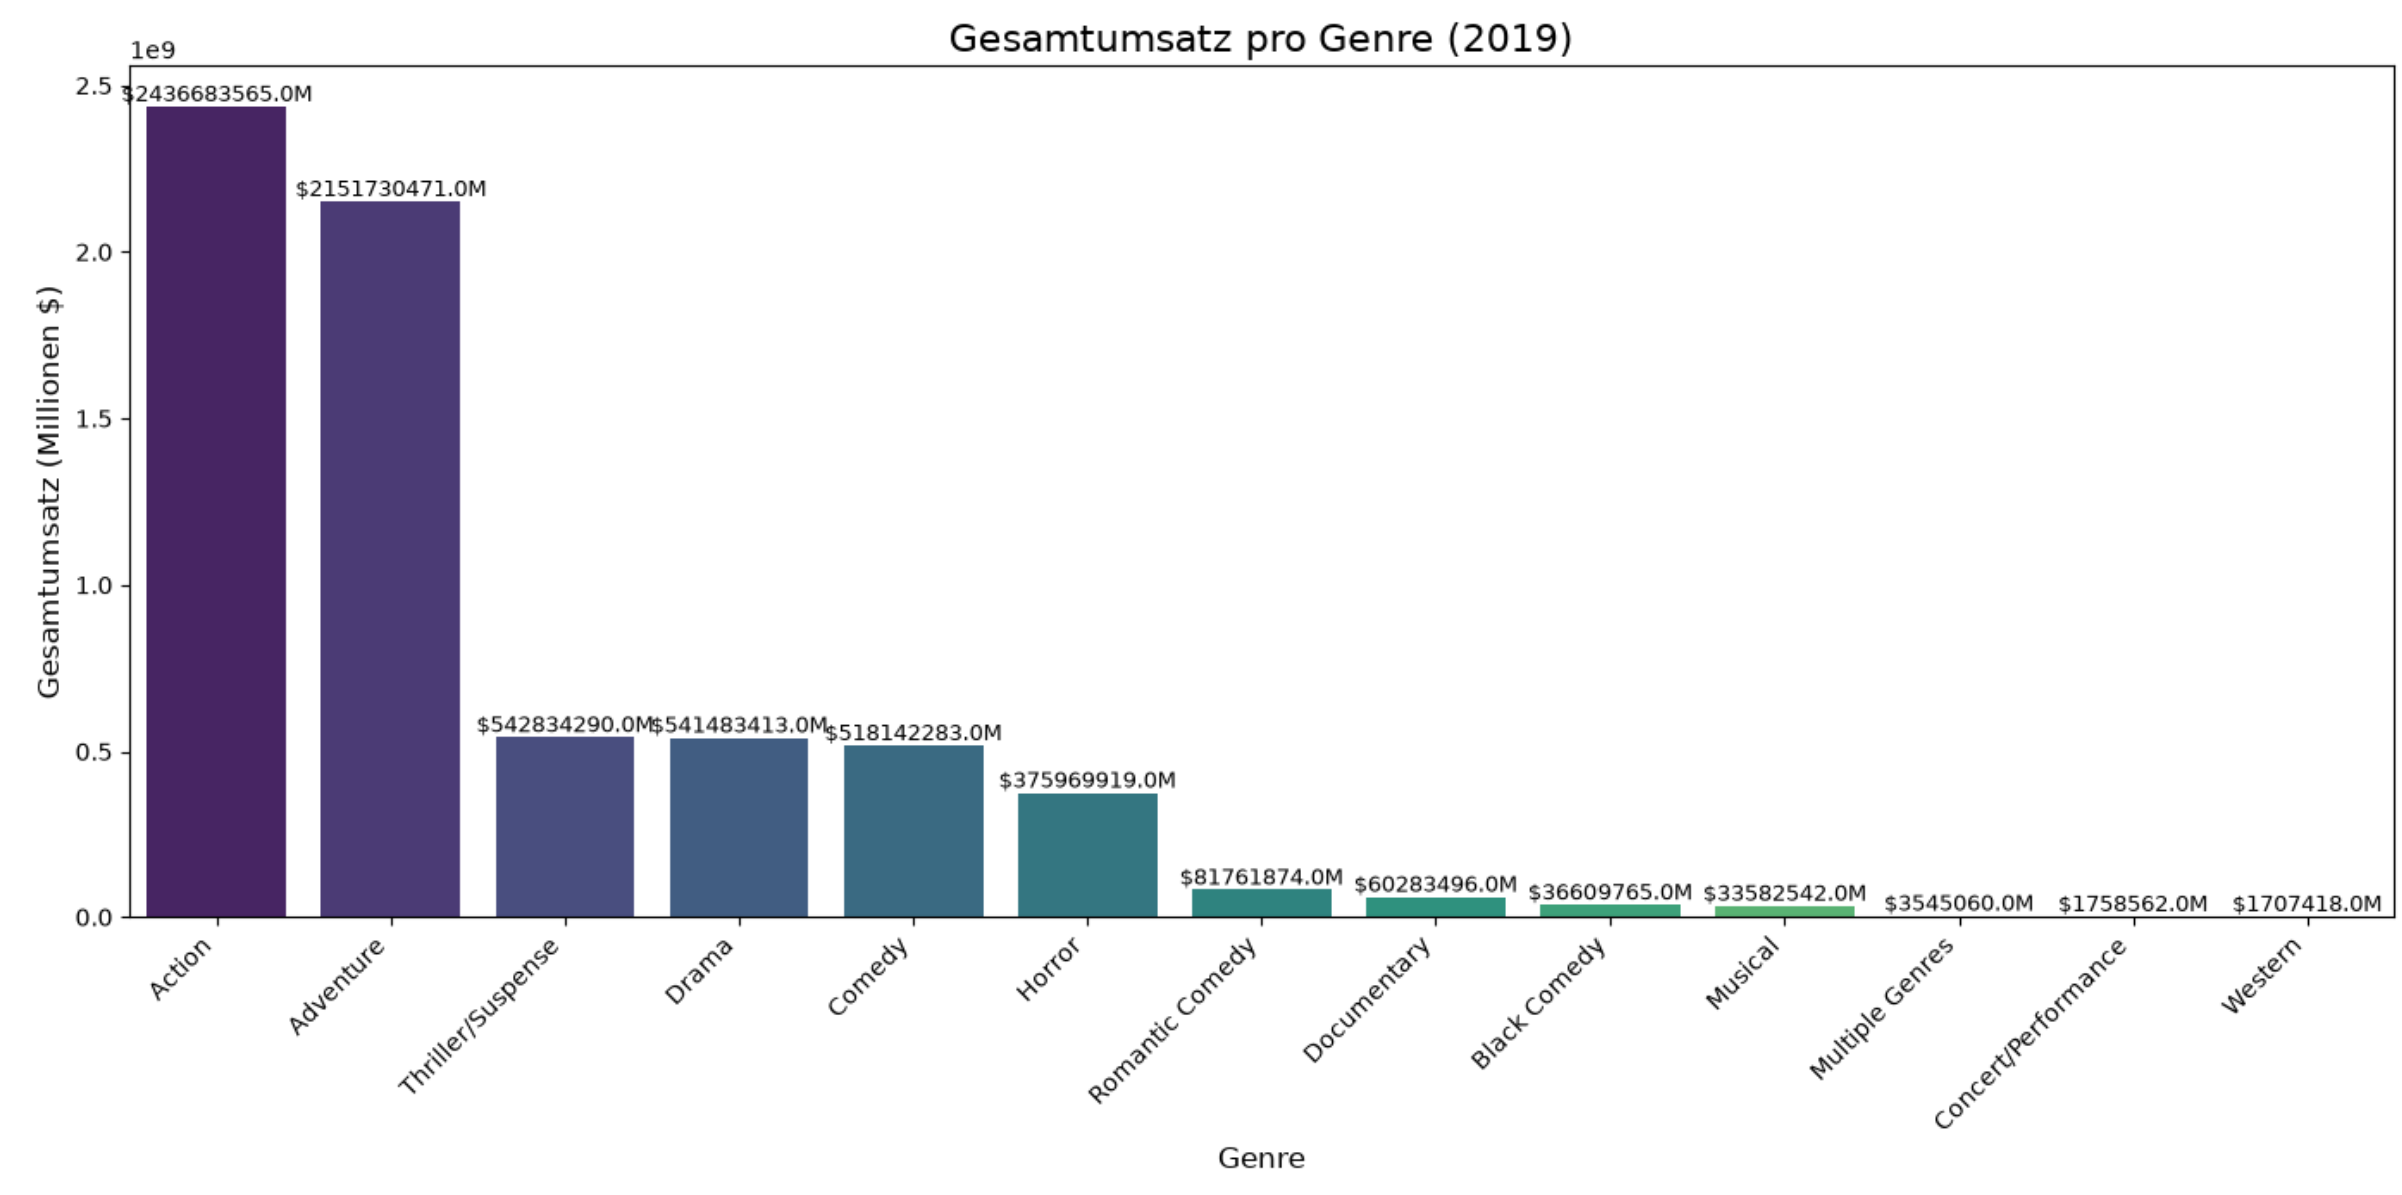
\includegraphics[width=0.9\textwidth]{./asset/image/Aufgabe1e.png}
    \caption{Barplot: Gesamtumsatz pro Genre (\textit{Quelle: Eigene Darstellung})}
    \label{fig:aufgabe1e}
\end{figure}

\subsection{Interpretation}

Die Daten werden mit \texttt{groupby(\textit{'Genre'})['2019 Gross'].sum()} aggregiert und mit \texttt{sort\_values(\textit{ascending=False})} absteigend sortiert, um die Genres mit dem höchsten Umsatz zuerst darzustellen. Der Barplot wird mit \texttt{sns.barplot()} erstellt, wobei die x-Achse die Genres und die y-Achse den Gesamtumsatz in Millionen USD abbildet. Die Plot-Größe wird mit \texttt{figsize=(\textit{14,7})} an die Anzahl der Genres angepasst, um überlappende Achsenbeschriftungen zu vermeiden. Die Umsatzwerte werden mit \texttt{plt.text()} über den Balken eingeblendet, um eine direkte Vergleichbarkeit der Werte zu ermöglichen. Die x-Achsen-Beschriftungen werden mit \texttt{plt.xticks(\textit{rotation=45})} gedreht, um die Lesbarkeit zu verbessern.

\cleardoublepage

% ======================================= f =====================================

\section{Barplot: Gesamtumsatz nach Monat (f)}
\label{sec:1f}

\subsection{Aufgabenstellung}

Es wird ein Barplot erstellt, der den Gesamtumsatz der Filme nach dem Monat der Veröffentlichung visualisiert. Dazu ist eine Transformation der Spalte \texttt{Release Date} erforderlich, um den Monat zu extrahieren.

\subsection{Lösung}

Zunächst wird die Spalte \texttt{Release Date} mit \texttt{pd.to\_datetime()} in ein Datumsformat konvertiert. Anschließend wird mit \texttt{dt.month} der Monat extrahiert und in einer neuen Spalte \texttt{Month} gespeichert. Für eine bessere Lesbarkeit werden die Monatsnamen (\textit{Jan–Dez}) in einer neuen Spalte \texttt{Month Name} zugeordnet. Die Gruppierung und Summierung der Umsätze pro Monat erfolgt mit \texttt{groupby()} und \texttt{sum()}. Der Barplot wird mit \texttt{sns.barplot()} erstellt, wobei die Monate auf der x-Achse und die Umsätze auf der y-Achse abgetragen werden. Die Plot-Größe wird mit \texttt{figsize=(\textit{14,7})} angepasst. Zusätzlich werden die Umsatzwerte über den Balken eingeblendet.

\lstinputlisting[
    language=Python, 
    caption={Barplot: Gesamtumsatz nach Monat}, 
    label={lst:aufgabe1f}
]{asset/code/Aufgabe1f.tex}

\subsection{Ausgabe}

Die Ausgabe zeigt den Gesamtumsatz pro Monat als Balkendiagramm:

\begin{figure}[h]
    \centering
    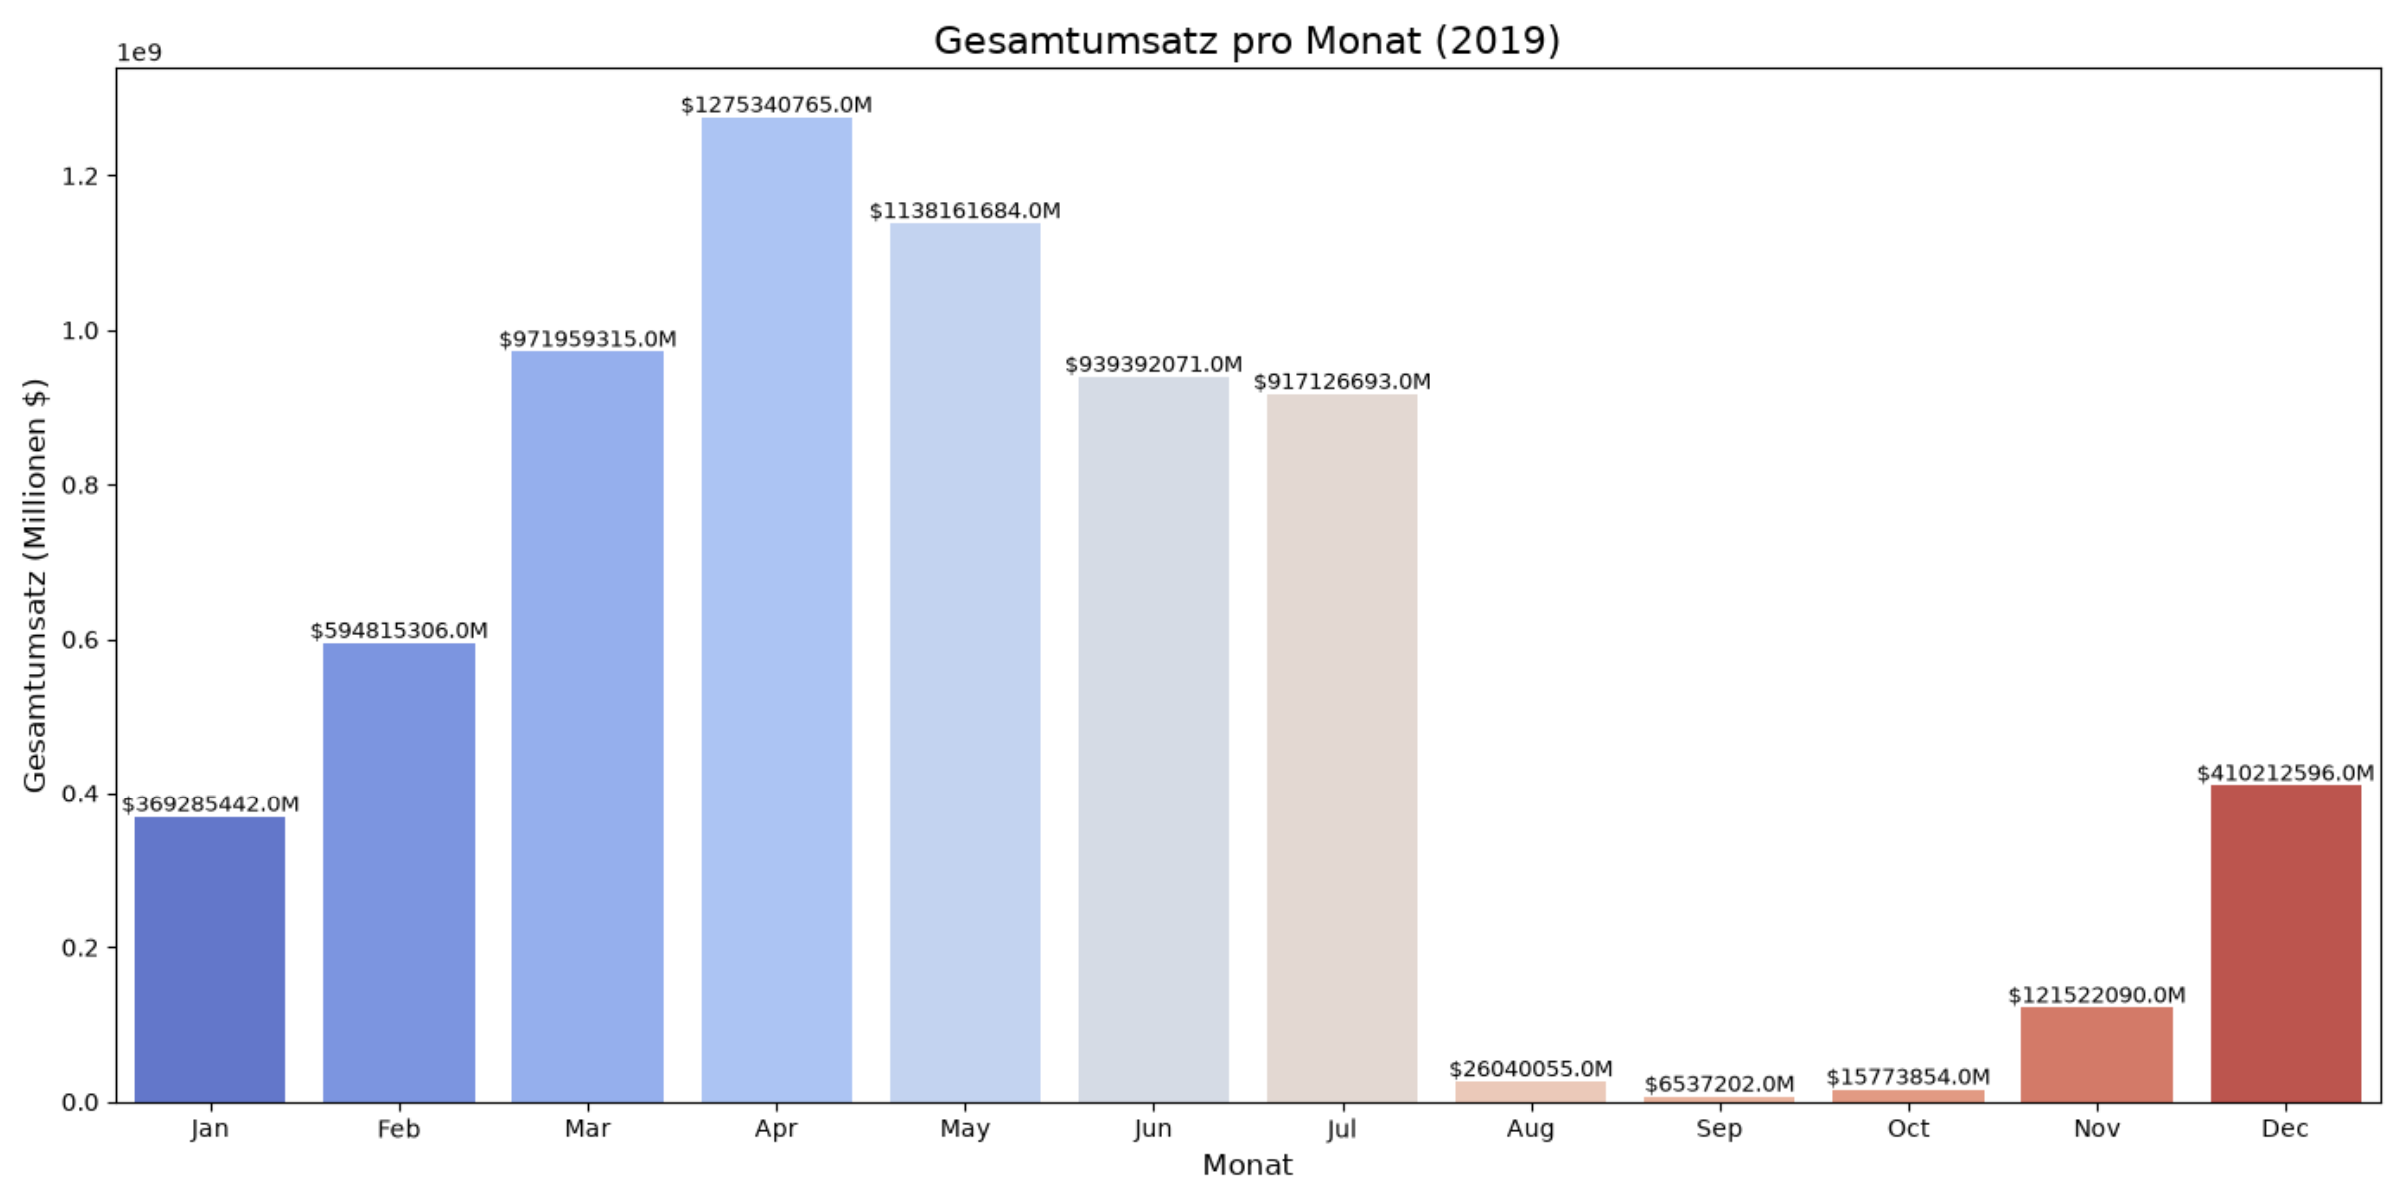
\includegraphics[width=0.9\textwidth]{./asset/image/Aufgabe1f.png}
    \caption{Barplot: Gesamtumsatz nach Monat (\textit{Quelle: Eigene Darstellung})}
    \label{fig:aufgabe1f}
\end{figure}

\subsection{Interpretation}

Die Spalte \texttt{Release Date} wird mit \texttt{pd.to\_datetime()} in ein Datumsformat konvertiert. Anschließend wird der Monat mit \texttt{dt.month} extrahiert und in einer neuen Spalte gespeichert. Die Monatsnamen werden über eine Abbildungsfunktion zugewiesen, um die Lesbarkeit der x-Achse zu verbessern. Die Gruppierung erfolgt mit \texttt{groupby(\textit{'Month'})['2019 Gross'].sum().sort\_index()}, wobei \texttt{sort\_index()} sicherstellt, dass die Monate in der korrekten chronologischen Reihenfolge dargestellt werden. Der Barplot wird mit \texttt{sns.barplot()} erstellt, wobei die x-Achse die Monate und die y-Achse den Gesamtumsatz in Millionen \acs{USD} abbildet. Die Werte werden mit \texttt{plt.text()} über den Balken eingeblendet, um die Vergleichbarkeit zu verbessern.

\cleardoublepage

% ======================================= g =====================================

\section{Top 5 Distributoren nach Gesamtumsatz (g)}
\label{sec:1g}

\subsection{Aufgabenstellung}

Die Gesamtumsätze werden nach Distributor gruppiert und absteigend sortiert. Die fünf Distributoren mit dem größten Gesamtumsatz werden ermittelt und genannt.

\subsection{Lösung}

Die Gruppierung erfolgt mit \texttt{groupby()} auf der Spalte \texttt{Distributor}. Die Summe der Umsätze pro Distributor wird mit \texttt{sum()} berechnet und mit \texttt{sort\_values(\textit{ascending=False})} absteigend sortiert. Die fünf größten Distributoren werden mit \texttt{head(\textit{5})} ausgewählt und ausgegeben.

\lstinputlisting[
    language=Python, 
    caption={Top 5 Distributoren nach Gesamtumsatz}, 
    label={lst:aufgabe1g}
]{asset/code/Aufgabe1g.tex}

\subsection{Ausgabe}

Die Ausgabe zeigt die fünf Distributoren mit dem höchsten Gesamtumsatz:

\begin{verbatim}
Top 5 Distributoren nach Gesamtumsatz 2019:
Distributor
Walt Disney      2.611281e+09
Warner Bros.     9.055731e+08
Universal        8.802197e+08
Sony Pictures    7.057896e+08
Lionsgate        3.930409e+08
Name: 2019 Gross, dtype: float64

Detaillierte Ausgabe:
1. Walt Disney: $2,611,280,507.00M
2. Warner Bros.: $905,573,135.00M
3. Universal: $880,219,708.00M
4. Sony Pictures: $705,789,563.00M
5. Lionsgate: $393,040,895.00M
\end{verbatim}

\subsection{Interpretation}

Die Gruppierung erfolgt mit \texttt{groupby(\textit{'Distributor'})['2019 Gross'].sum()}, um die Gesamtumsätze pro Distributor zu berechnen. Die Sortierung mit \\ \texttt{sort\_values(\textit{ascending=False})} ordnet die Distributoren absteigend nach Umsatz, sodass der umsatzstärkste Distributor an erster Stelle steht. Mit \texttt{head(\textit{5})} werden die fünf größten Distributoren ausgewählt. Die Ausgabe zeigt, dass \texttt{Walt Disney} den höchsten Gesamtumsatz erzielt hat, gefolgt von \texttt{Warner Bros.}, \texttt{Universal}, \texttt{Sony Pictures} und \texttt{Lionsgate}.

\cleardoublepage

% ======================================= h =====================================

\section{Fehlende Information zur Erfolgsbeurteilung (h)}
\label{sec:1h}

\subsection{Aufgabenstellung}

Es wird analysiert, welche Information im Datensatz fehlt, um den "Erfolg" eines Distributors vollständig beurteilen zu können.

\subsection{Lösung}

Der Datensatz enthält den Umsatz (\textit{\texttt{2019 Gross}}) der Filme, jedoch keine Angaben zu den Produktionskosten. Ohne die Kosten ist eine Beurteilung des wirtschaftlichen Erfolgs nicht möglich, da der Gewinn erst aus der Differenz von Umsatz und Kosten berechnet werden kann.

Folgende Informationen fehlen für eine vollständige Erfolgsbeurteilung:

\begin{itemize}
    \item \textbf{Produktionskosten (\textit{Budget}):} Die Herstellungskosten der Filme sind nicht enthalten. Ein Film mit hohem Umsatz kann dennoch ein Verlustgeschäft sein, wenn die Produktionskosten den Umsatz übersteigen.
    \item \textbf{Marketingkosten:} Die Ausgaben für Werbung und Vermarktung sind nicht erfasst. Diese können einen erheblichen Teil des Umsatzes aufzehren.
    \item \textbf{Rentabilität (\textit{Return on Investment}):} Ohne Kostenangaben kann die Rentabilität nicht berechnet werden. Der Erfolg eines Distributors bemisst sich nicht allein am Umsatz, sondern an der erzielten Marge.
    \item \textbf{Anzahl der veröffentlichten Filme:} Ein Distributor mit wenigen, aber sehr erfolgreichen Filmen kann wirtschaftlich erfolgreicher sein als ein Distributor mit vielen, aber weniger profitablen Filmen.
    \item \textbf{Zusätzliche Einnahmequellen:} Einnahmen aus Merchandising, Streaming-Rechten, internationalen Verkäufen oder Home-Entertainment sind nicht enthalten.
\end{itemize}

\subsection{Interpretation}

Der Datensatz ermöglicht eine Umsatzanalyse, jedoch keine vollständige Erfolgsbeurteilung. Der wirtschaftliche Erfolg eines Distributors wird nicht allein durch den Umsatz bestimmt, sondern durch die erzielte Gewinnmarge. Hierfür sind die Produktions- und Marketingkosten sowie zusätzliche Einnahmequellen erforderlich. Die fehlenden Kosteninformationen machen eine Aussage über die tatsächliche Profitabilität der Distributoren unmöglich.

% ==============================================================================
% =============================== Ende Aufgabe 1 ===============================
% ==============================================================================